\documentclass{standalone}
\usepackage{tikz}
\usetikzlibrary{patterns, positioning}


\begin{document}
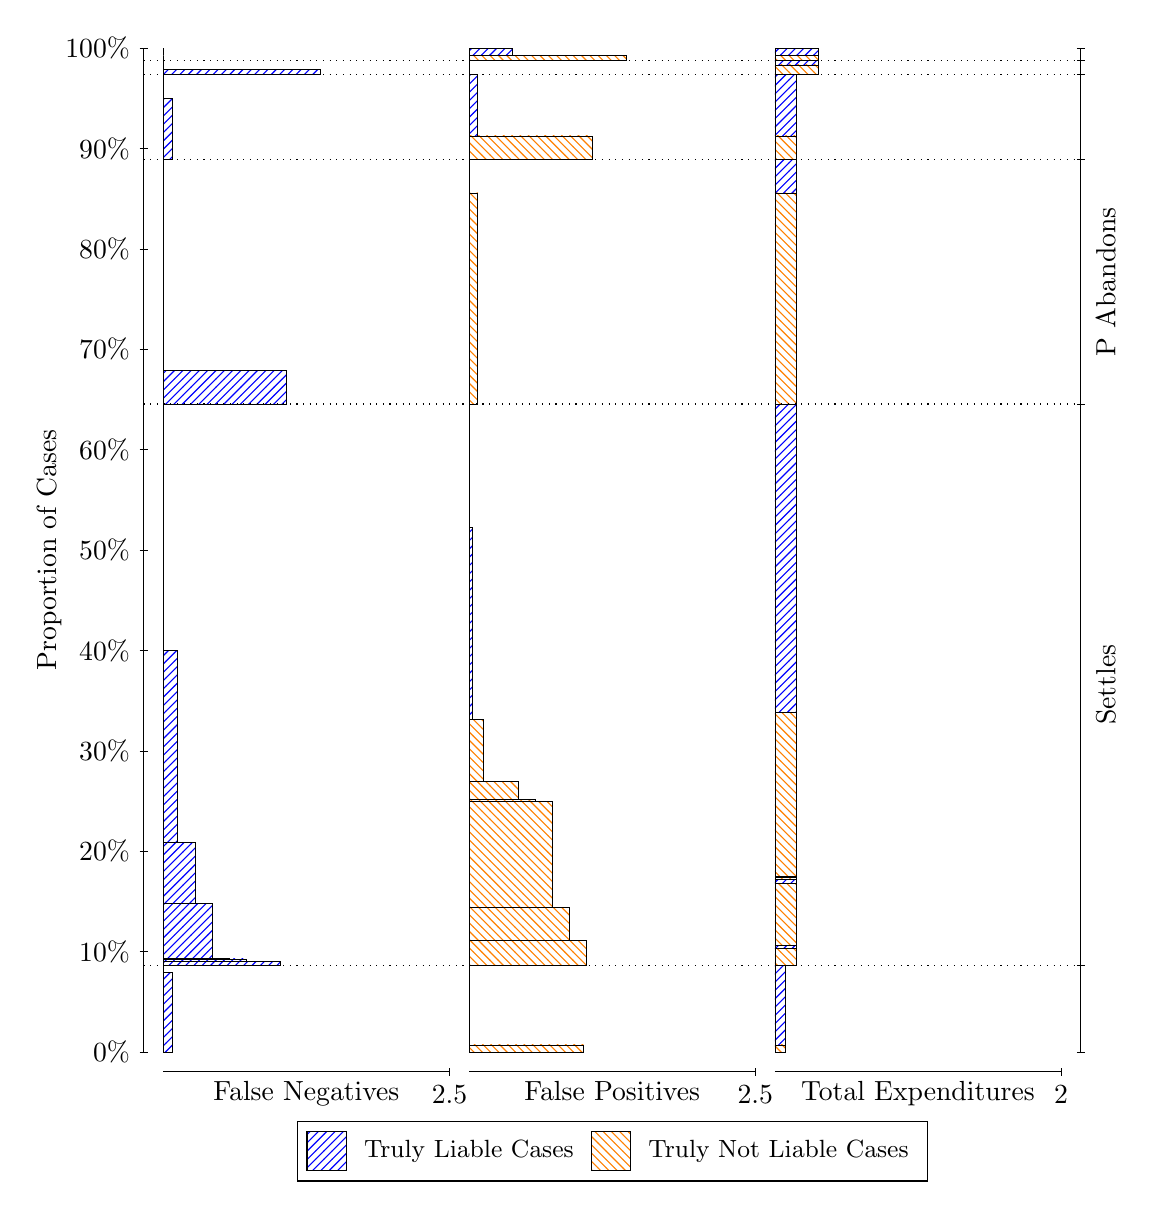
\begin{tikzpicture}
\draw[black, very thin] (1.5,1.75) -- (1.5,14.5);
\node[rotate=90, text=black, anchor=center] at (0.3, 8.125) {Proportion of Cases};
\draw[black, very thin] (1.45,1.75) -- (1.55,1.75);
\node[text=black, anchor=east] at (1.45, 1.75) {0\%};
\draw[black, very thin] (1.45,3.025) -- (1.55,3.025);
\node[text=black, anchor=east] at (1.45, 3.025) {10\%};
\draw[black, very thin] (1.45,4.3) -- (1.55,4.3);
\node[text=black, anchor=east] at (1.45, 4.3) {20\%};
\draw[black, very thin] (1.45,5.575) -- (1.55,5.575);
\node[text=black, anchor=east] at (1.45, 5.575) {30\%};
\draw[black, very thin] (1.45,6.85) -- (1.55,6.85);
\node[text=black, anchor=east] at (1.45, 6.85) {40\%};
\draw[black, very thin] (1.45,8.125) -- (1.55,8.125);
\node[text=black, anchor=east] at (1.45, 8.125) {50\%};
\draw[black, very thin] (1.45,9.4) -- (1.55,9.4);
\node[text=black, anchor=east] at (1.45, 9.4) {60\%};
\draw[black, very thin] (1.45,10.675) -- (1.55,10.675);
\node[text=black, anchor=east] at (1.45, 10.675) {70\%};
\draw[black, very thin] (1.45,11.95) -- (1.55,11.95);
\node[text=black, anchor=east] at (1.45, 11.95) {80\%};
\draw[black, very thin] (1.45,13.225) -- (1.55,13.225);
\node[text=black, anchor=east] at (1.45, 13.225) {90\%};
\draw[black, very thin] (1.45,14.5) -- (1.55,14.5);
\node[text=black, anchor=east] at (1.45, 14.5) {100\%};

\draw[black, very thin] (13.4,1.75) -- (13.4,14.5);
\draw[black, very thin] (13.35,1.75) -- (13.45,1.75);
\node[anchor=west] at (13.35, 1.75) {};
\draw[black, very thin] (13.35,2.8497) -- (13.45,2.8497);
\node[anchor=west] at (13.35, 2.8497) {};
\draw[black, very thin] (13.35,9.9788) -- (13.45,9.9788);
\node[anchor=west] at (13.35, 9.9788) {};
\draw[black, very thin] (13.35,13.083) -- (13.45,13.083);
\node[anchor=west] at (13.35, 13.083) {};
\draw[black, very thin] (13.35,14.165) -- (13.45,14.165);
\node[anchor=west] at (13.35, 14.165) {};
\draw[black, very thin] (13.35,14.345) -- (13.45,14.345);
\node[anchor=west] at (13.35, 14.345) {};
\draw[black, very thin] (13.35,14.5) -- (13.45,14.5);
\node[anchor=west] at (13.35, 14.5) {};

\draw[black, very thin, pattern color=blue, pattern=north east lines] (1.75,1.75) rectangle (1.859,2.7607);
\draw[black, very thin, pattern color=orange, pattern=north west lines] (1.75,2.7607) rectangle (1.75,2.8497);
\draw[black, very thin, pattern color=blue, pattern=north east lines] (1.75,2.8497) rectangle (3.2397,2.9012);
\draw[black, very thin, pattern color=blue, pattern=north east lines] (1.75,2.9012) rectangle (2.8037,2.9318);
\draw[black, very thin, pattern color=blue, pattern=north east lines] (1.75,2.9318) rectangle (2.5857,2.9421);
\draw[black, very thin, pattern color=blue, pattern=north east lines] (1.75,2.9421) rectangle (2.3677,3.6395);
\draw[black, very thin, pattern color=blue, pattern=north east lines] (1.75,3.6395) rectangle (2.1497,4.4144);
\draw[black, very thin, pattern color=blue, pattern=north east lines] (1.75,4.4144) rectangle (1.9317,6.8535);
\draw[black, very thin, pattern color=orange, pattern=north west lines] (1.75,6.8535) rectangle (1.75,9.9788);
\draw[black, very thin, pattern color=blue, pattern=north east lines] (1.75,9.9788) rectangle (3.3123,10.403);
\draw[black, very thin, pattern color=orange, pattern=north west lines] (1.75,10.403) rectangle (1.75,13.083);
\draw[black, very thin, pattern color=blue, pattern=north east lines] (1.75,13.083) rectangle (1.859,13.865);
\draw[black, very thin, pattern color=orange, pattern=north west lines] (1.75,13.865) rectangle (1.75,14.165);
\draw[black, very thin, pattern color=blue, pattern=north east lines] (1.75,14.165) rectangle (3.7483,14.224);
\draw[black, very thin, pattern color=orange, pattern=north west lines] (1.75,14.224) rectangle (1.75,14.345);
\draw[black, very thin, pattern color=orange, pattern=north west lines] (1.75,14.345) rectangle (1.75,14.404);
\draw[black, very thin, pattern color=blue, pattern=north east lines] (1.75,14.404) rectangle (1.75,14.5);
\draw[black, very thin, pattern color=orange, pattern=north west lines] (5.6333,1.75) rectangle (7.0867,1.839);
\draw[black, very thin, pattern color=blue, pattern=north east lines] (5.6333,1.839) rectangle (5.6333,2.8497);
\draw[black, very thin, pattern color=orange, pattern=north west lines] (5.6333,2.8497) rectangle (7.123,3.1665);
\draw[black, very thin, pattern color=orange, pattern=north west lines] (5.6333,3.1665) rectangle (6.905,3.5889);
\draw[black, very thin, pattern color=orange, pattern=north west lines] (5.6333,3.5889) rectangle (6.687,4.935);
\draw[black, very thin, pattern color=orange, pattern=north west lines] (5.6333,4.935) rectangle (6.469,4.9622);
\draw[black, very thin, pattern color=orange, pattern=north west lines] (5.6333,4.9622) rectangle (6.251,5.1821);
\draw[black, very thin, pattern color=orange, pattern=north west lines] (5.6333,5.1821) rectangle (5.815,5.975);
\draw[black, very thin, pattern color=blue, pattern=north east lines] (5.6333,5.975) rectangle (5.6697,8.4141);
\draw[black, very thin, pattern color=blue, pattern=north east lines] (5.6333,8.4141) rectangle (5.6333,9.9788);
\draw[black, very thin, pattern color=orange, pattern=north west lines] (5.6333,9.9788) rectangle (5.7423,12.659);
\draw[black, very thin, pattern color=blue, pattern=north east lines] (5.6333,12.659) rectangle (5.6333,13.083);
\draw[black, very thin, pattern color=orange, pattern=north west lines] (5.6333,13.083) rectangle (7.1957,13.384);
\draw[black, very thin, pattern color=blue, pattern=north east lines] (5.6333,13.384) rectangle (5.7423,14.165);
\draw[black, very thin, pattern color=orange, pattern=north west lines] (5.6333,14.165) rectangle (5.6333,14.287);
\draw[black, very thin, pattern color=blue, pattern=north east lines] (5.6333,14.287) rectangle (5.6333,14.345);
\draw[black, very thin, pattern color=orange, pattern=north west lines] (5.6333,14.345) rectangle (7.6317,14.404);
\draw[black, very thin, pattern color=blue, pattern=north east lines] (5.6333,14.404) rectangle (6.1783,14.5);
\draw[black, very thin, pattern color=orange, pattern=north west lines] (9.5167,1.75) rectangle (9.6529,1.839);
\draw[black, very thin, pattern color=blue, pattern=north east lines] (9.5167,1.839) rectangle (9.6529,2.8497);
\draw[black, very thin, pattern color=orange, pattern=north west lines] (9.5167,2.8497) rectangle (9.7892,3.0697);
\draw[black, very thin, pattern color=blue, pattern=north east lines] (9.5167,3.0697) rectangle (9.7892,3.1004);
\draw[black, very thin, pattern color=orange, pattern=north west lines] (9.5167,3.1004) rectangle (9.7892,3.8933);
\draw[black, very thin, pattern color=blue, pattern=north east lines] (9.5167,3.8933) rectangle (9.7892,3.9447);
\draw[black, very thin, pattern color=orange, pattern=north west lines] (9.5167,3.9447) rectangle (9.7892,3.9719);
\draw[black, very thin, pattern color=blue, pattern=north east lines] (9.5167,3.9719) rectangle (9.7892,3.9822);
\draw[black, very thin, pattern color=orange, pattern=north west lines] (9.5167,3.9822) rectangle (9.7892,6.0674);
\draw[black, very thin, pattern color=blue, pattern=north east lines] (9.5167,6.0674) rectangle (9.7892,9.9788);
\draw[black, very thin, pattern color=orange, pattern=north west lines] (9.5167,9.9788) rectangle (9.7892,12.659);
\draw[black, very thin, pattern color=blue, pattern=north east lines] (9.5167,12.659) rectangle (9.7892,13.083);
\draw[black, very thin, pattern color=orange, pattern=north west lines] (9.5167,13.083) rectangle (9.7892,13.384);
\draw[black, very thin, pattern color=blue, pattern=north east lines] (9.5167,13.384) rectangle (9.7892,14.165);
\draw[black, very thin, pattern color=orange, pattern=north west lines] (9.5167,14.165) rectangle (10.062,14.287);
\draw[black, very thin, pattern color=blue, pattern=north east lines] (9.5167,14.287) rectangle (10.062,14.345);
\draw[black, very thin, pattern color=orange, pattern=north west lines] (9.5167,14.345) rectangle (10.062,14.404);
\draw[black, very thin, pattern color=blue, pattern=north east lines] (9.5167,14.404) rectangle (10.062,14.5);
\draw[black, dotted] (1.5,2.8497) -- (13.4,2.8497);
\draw[black, dotted] (1.5,9.9788) -- (13.4,9.9788);
\draw[black, dotted] (1.5,13.083) -- (13.4,13.083);
\draw[black, dotted] (1.5,14.165) -- (13.4,14.165);
\draw[black, dotted] (1.5,14.345) -- (13.4,14.345);
\draw[black, very thin] (1.75,1.5) -- (5.3833,1.5);
\node[text=black, anchor=north] at (3.5667, 1.5) {False Negatives};
\draw[black, very thin] (5.3833,1.45) -- (5.3833,1.55);
\node[text=black, anchor=north] at (5.3833, 1.45) {2.5};

\draw[black, very thin] (5.6333,1.5) -- (9.2667,1.5);
\node[text=black, anchor=north] at (7.45, 1.5) {False Positives};
\draw[black, very thin] (9.2667,1.45) -- (9.2667,1.55);
\node[text=black, anchor=north] at (9.2667, 1.45) {2.5};

\draw[black, very thin] (9.5167,1.5) -- (13.15,1.5);
\node[text=black, anchor=north] at (11.333, 1.5) {Total Expenditures};
\draw[black, very thin] (13.15,1.45) -- (13.15,1.55);
\node[text=black, anchor=north] at (13.15, 1.45) {2};


\node[text=black, centered, rotate=90] at (13.72, 6.4143) {Settles};
\node[text=black, centered, rotate=90] at (13.72, 11.531) {P Abandons};




\draw (7.449999999999999,1.5) node[draw=none] (baseCoordinate) {};
\begin{scope}[align=center]
        \matrix[scale=0.5, draw=black, below=0.5cm of baseCoordinate, nodes={draw}, column sep=0.1cm]{
            \node[rectangle, draw, minimum width=0.5cm, minimum height=0.5cm, pattern color=blue, pattern=north east lines] {}; &
            \node[draw=none, font=\small, text=black] (B) {Truly Liable Cases}; &
            \node[rectangle, draw, minimum width=0.5cm, minimum height=0.5cm, pattern color=orange, pattern=north west lines] {}; &
            \node[draw=none, font=\small, text=black] (B) {Truly Not Liable Cases}; \\
            };
\end{scope}

\end{tikzpicture}
\end{document}